\documentclass[a4paper,12pt]{jarticle}
\input ./chap01_preamble.tex
\graphicspath{%
  {../text01-img/}%
}
% !TEX root = ./chap01_07.tex
\begin{document}
\section{\ruby{解答}{かいとう}例}
 {Figure~\ref{seq:refFigure43}はしゅみの\ruby{紹介}{しょうかい}のホームページの例です。HTMLファイルは01フォルダのsample3.htmlです。参考に\ruby{確認}{かくにん}しましょう。}\\
{Figure~\ref{seq:refFigure44}は学校紹介のホームページの例です。HTMLファイルは01フォルダのsample2.htmlです。参考に確認しましょう。}\\
{Figure~\ref{seq:refFigure45}は\ruby{時間割}{じかんわり}表の例です。HTMLファイルは01フォルダのsample1.htmlです。参考に確認しましょう。}\\

\centering
\begin{minipage}{7.518cm}
  {\upshape
    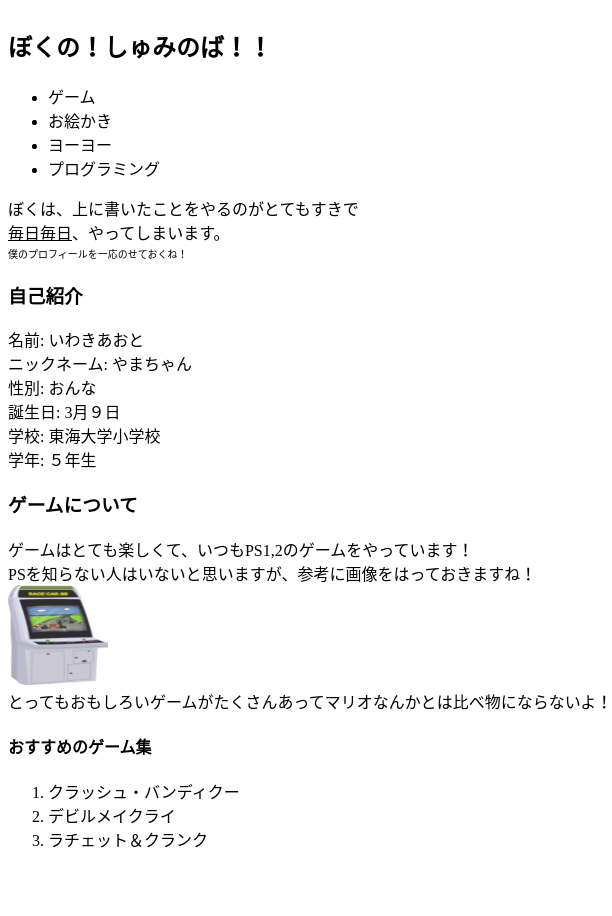
\includegraphics[width=6.525cm,height=8.262cm]{textbook-img209.png}
    \newline
    Figure {\refstepcounter{Figure}\theFigure\label{seq:refFigure43}}:
    \ruby{趣味}{しゅみ}ホームページサンプル}
\end{minipage}
\begin{minipage}{7.703cm}
  {\upshape
    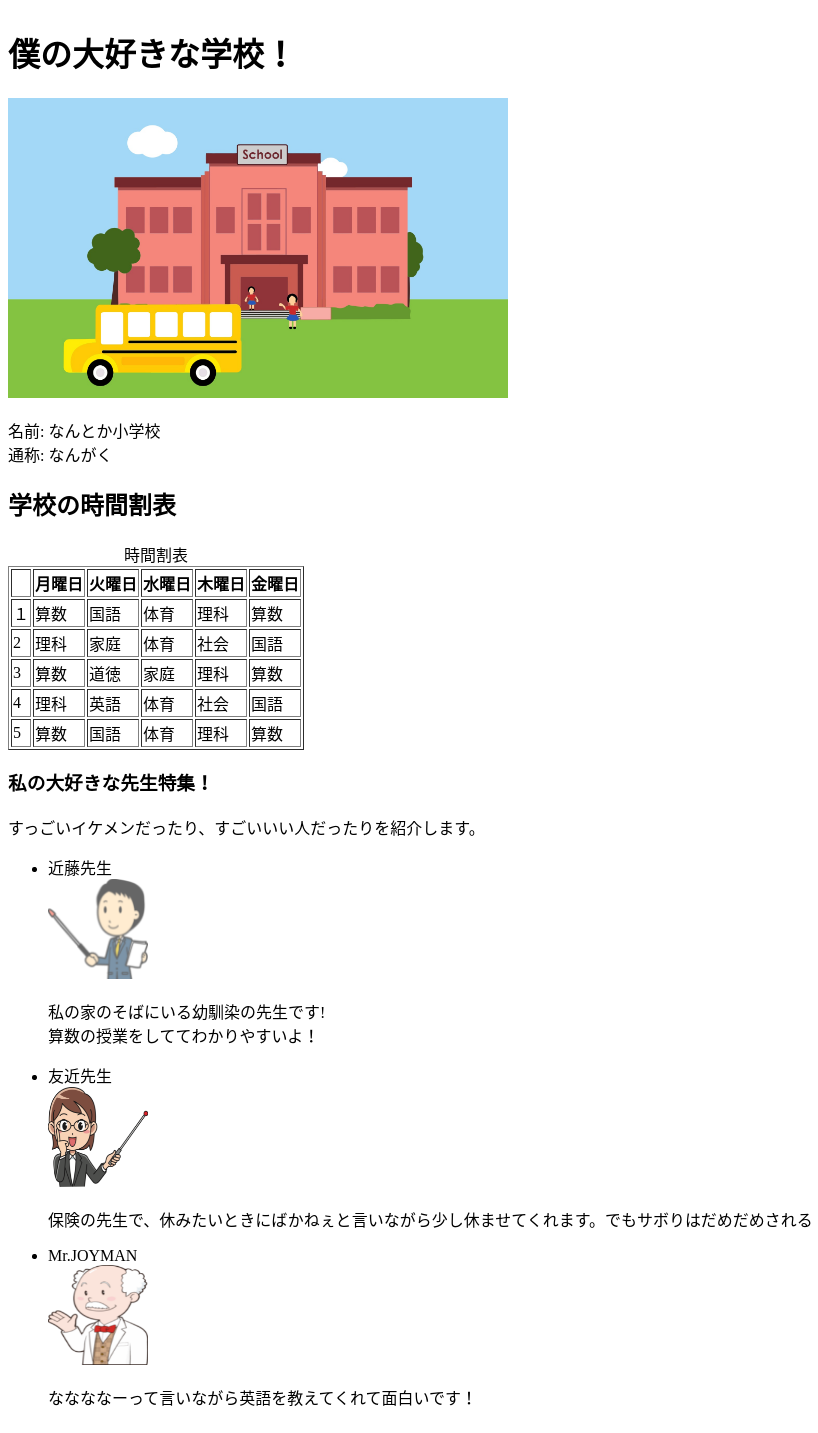
\includegraphics[width=6.062cm,height=9.306cm]{textbook-img210.png}
    \newline
    Figure {\refstepcounter{Figure}\theFigure\label{seq:refFigure44}}:
    学校紹介ホームページサンプル}
\end{minipage}
\begin{minipage}{6.839cm}
  {\upshape
    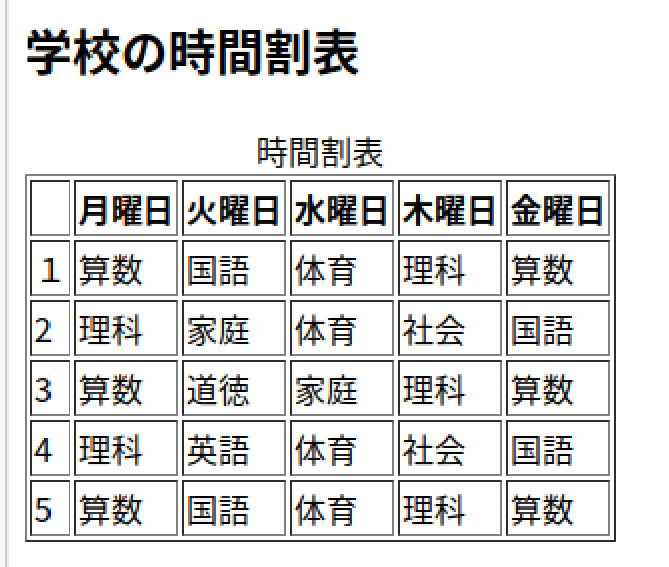
\includegraphics[width=6.839cm,height=5.727cm]{textbook-img211.png}
    \newline
    Figure {\refstepcounter{Figure}\theFigure\label{seq:refFigure45}}:
    時間割表サンプル}
\end{minipage}

\bigskip

\flushleft
\clearpage\subsection{\bfseries
  問題の答え}

問題の答えをのせてあります。まずは答えをみないで\ruby{解}{と}いていきましょう。\newline
問題の答えがないところは例題とほぼ変わらないためはぶいています。

\subsubsection{\bfseries
  \ref*{Q:hasAnswer02-1}答え}

\bigskip


\centering
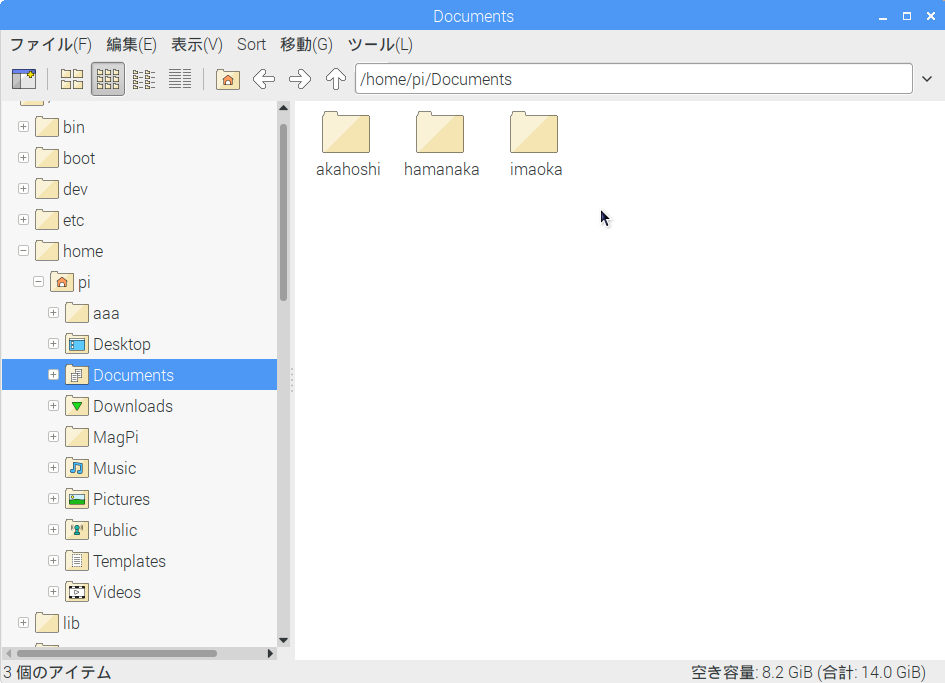
\includegraphics[width=9.763cm,height=8.038cm]{textbook-img212.png}
\flushleft

\bigskip


\bigskip


\bigskip

\subsubsection{\bfseries
\ref*{Q:hasAnswer02-2}答え}

\bigskip



\centering
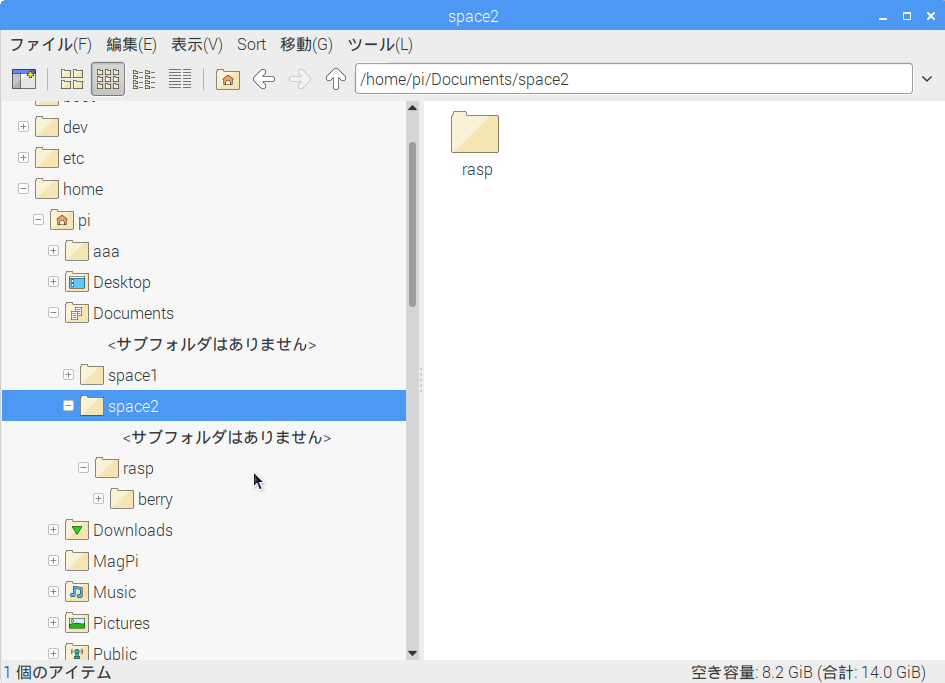
\includegraphics[width=11.081cm,height=8.008cm]{textbook-img213.png}
\flushleft

\clearpage\subsubsection{\bfseries
\ref*{Q:hasAnswer02-3}答え}


\begin{enumerate}
  \item
        miss\_nameフォルダの上で右クリックしてファイル名の\ruby{変更}{へんこう}をクリック

        \centering
        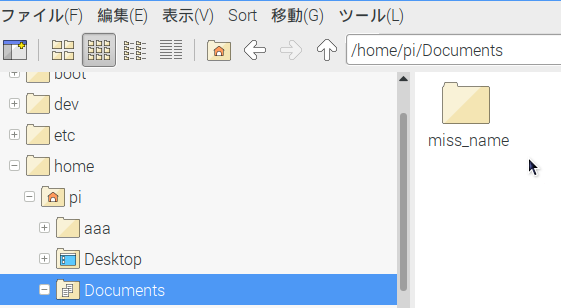
\includegraphics[width=7.913cm,height=4.344cm]{textbook-img214.png}
        \flushleft

  \item success\_nameに変更

        \centering
        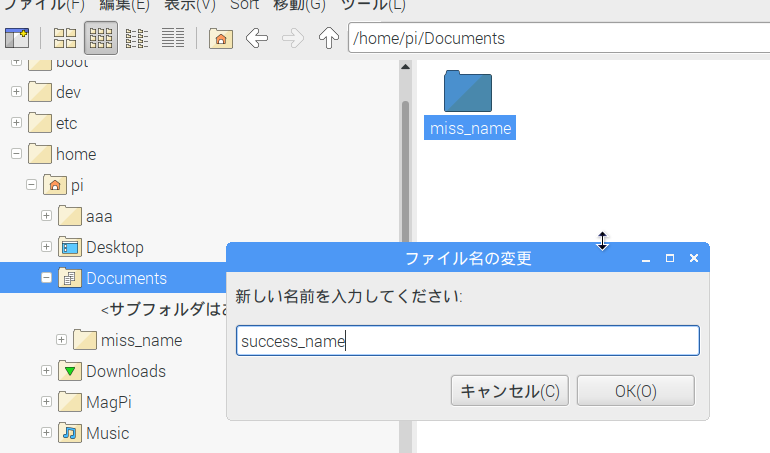
\includegraphics[width=8.694cm,height=5.115cm]{textbook-img215.png}
        \flushleft
  \item success\_nameに変更できました

        \centering
        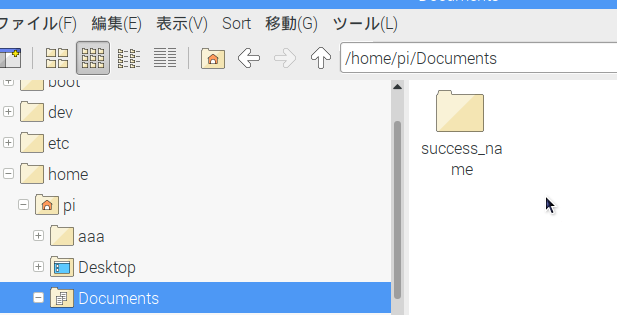
\includegraphics[width=8.895cm,height=4.542cm]{textbook-img216.png}
        \flushleft
\end{enumerate}



\subsubsection{\bfseries
\ref*{Q:hasAnswer02-4}答え}

shiftキーを\ruby{押}{お}しながら、アルファベットキーを打つと大文字入力になるよ


\centering
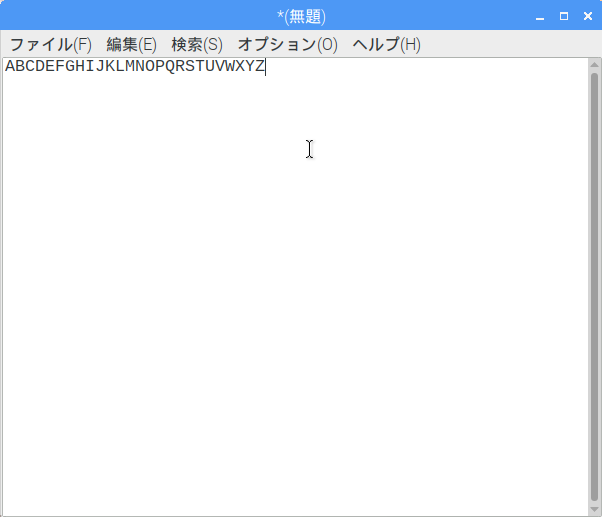
\includegraphics[width=10.031cm,height=2.27cm]{textbook-img217.png}
\flushleft

\clearpage\subsubsection{\bfseries
\ref*{Q:hasAnswer02-5}答え}

右上にキーボードマークが出ていることを確認しよう。そのじょうたいで入力しよう。


\bigskip


\centering
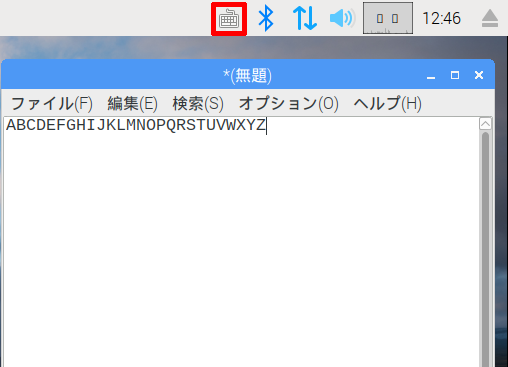
\includegraphics[width=10.075cm,height=3.914cm]{textbook-img218.png}
\flushleft


\bigskip





\centering
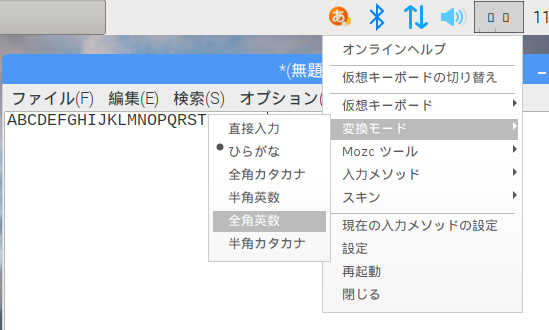
\includegraphics[width=9.733cm,height=5.851cm]{textbook-img219.png}
\flushleft


\bigskip

{\bfseries
  半角大文字でアルファベットの入力を終えたら右上のキーボードマークをクリックし

  「あ」マークにして右クリックし、\ruby{変換}{へんかん}モードから全角英数をクリック}



\bigskip

\bigskip


\centering
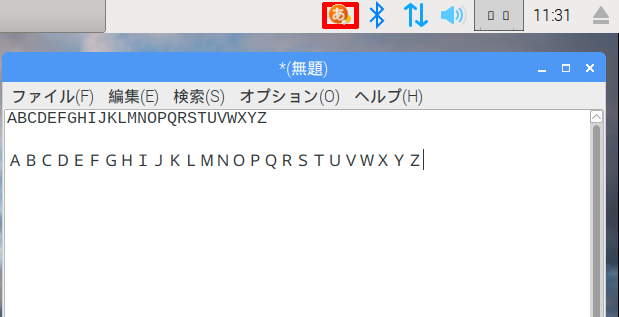
\includegraphics[width=12.631cm,height=4.297cm]{textbook-img220.png}
\flushleft

\bigskip

全角アルファベットを入力しよう。
\clearpage

\subsubsection{\bfseries
\ref*{Q:hasAnswer02-6}答え}

参考にして、じぶんの好きな\ruby{画像}{がぞう}を\ruby{保存}{ほぞん}しよう。

\centering
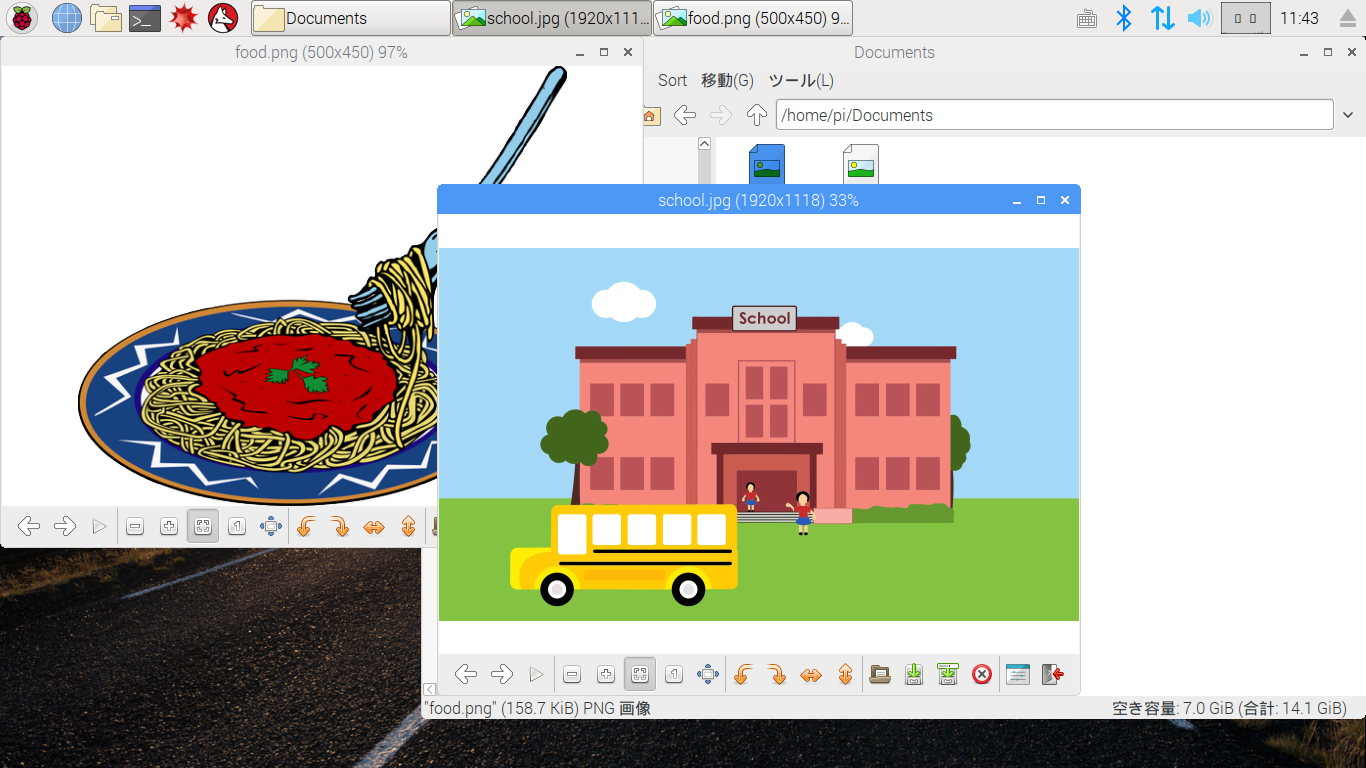
\includegraphics[width=11.705cm,height=6.581cm]{textbook-img221.png}
\flushleft

\bigskip


\subsubsection{\bfseries
\ref*{Q:hasAnswer02-7}答え}



\centering
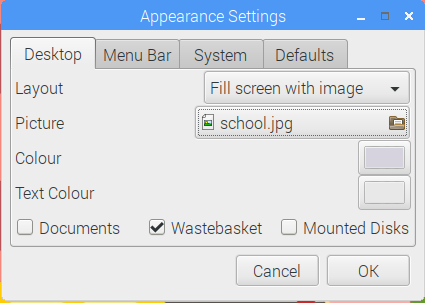
\includegraphics[width=7.631cm,height=5.44cm]{textbook-img222.png}


\centering
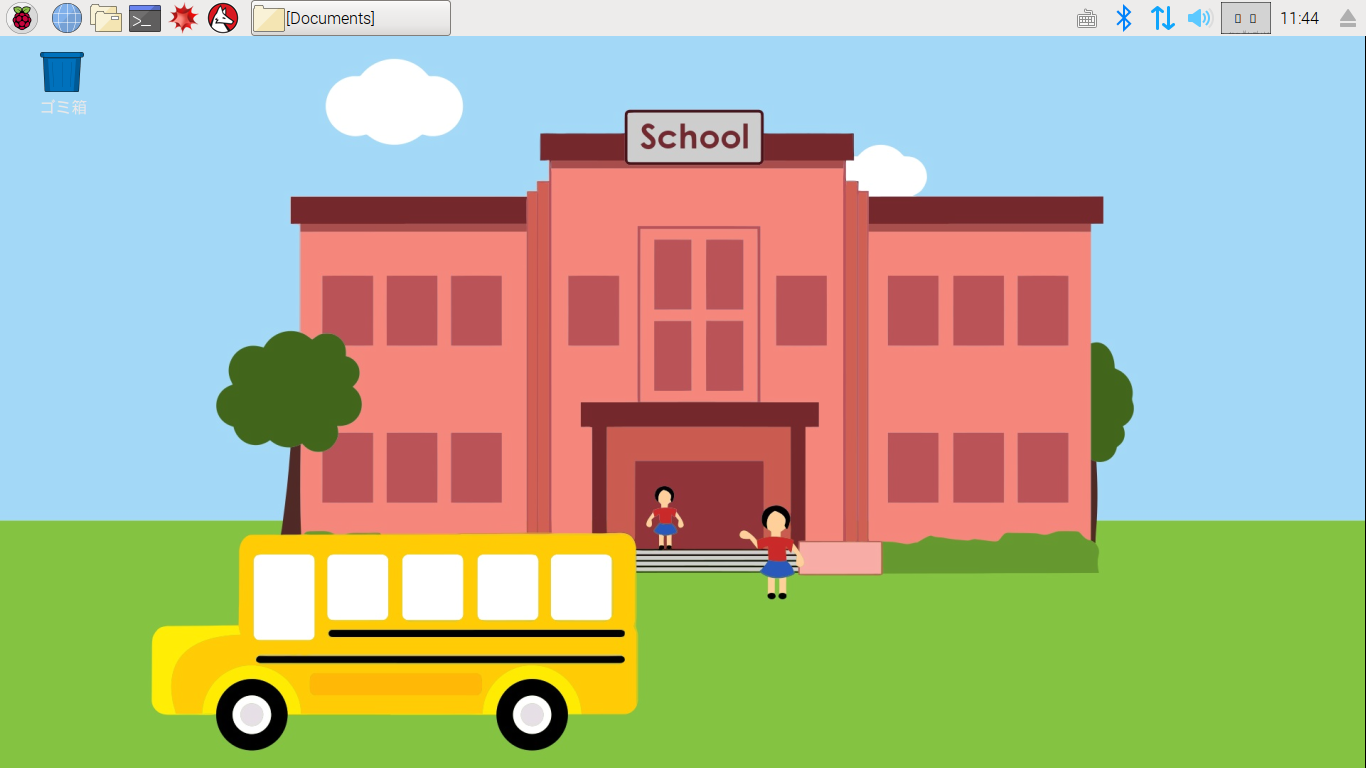
\includegraphics[width=11.621cm,height=6.533cm]{textbook-img223.png}


\flushleft
\clearpage
\begin{minipage}{\textwidth}
  \subsubsection{\bfseries
  \ref*{Q:hasAnswer04-1}答え}

  \centering
  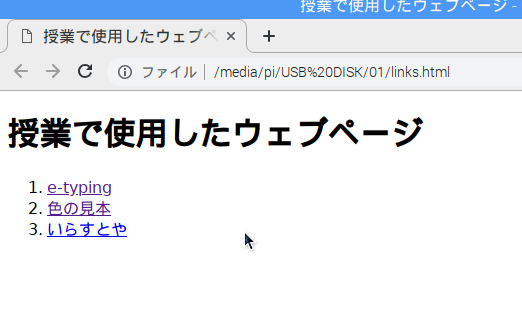
\includegraphics[width=7.0cm,height=3.5cm]{textbook-img224.png}
  \flushleft

  \subsubsection{\bfseries
  \ref*{Q:hasAnswer04-2}答え}

  \begin{center}
    \tablefirsthead{}
    \tablehead{}
    \tabletail{}
    \tablelasttail{}
    \begin{supertabular}{|m{5.467cm}|m{5.4690003cm}|m{5.4690003cm}}
      \hline
      \centering
      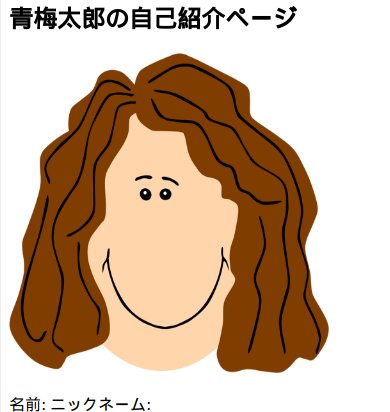
\includegraphics[width=5.373cm,height=5.579cm]{textbook-img225.png}
      &
      \centering
      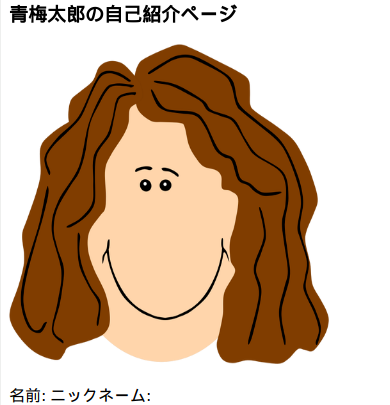
\includegraphics[width=5.373cm,height=5.579cm]{textbook-img226.png}
      &
      \multicolumn{1}{m{5.4690003cm}|}{\centering\arraybslash
        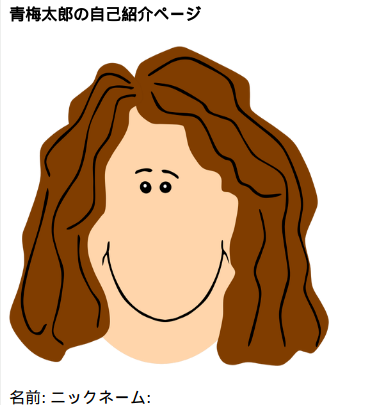
\includegraphics[width=5.373cm,height=5.579cm]{textbook-img227.png}
        \flushleft

        \bigskip
      }\\\hline
      \centering h2 &
      \centering h3 &
      \multicolumn{1}{m{5.4690003cm}|}{\centering\arraybslash h4}\\\hline
      \centering
      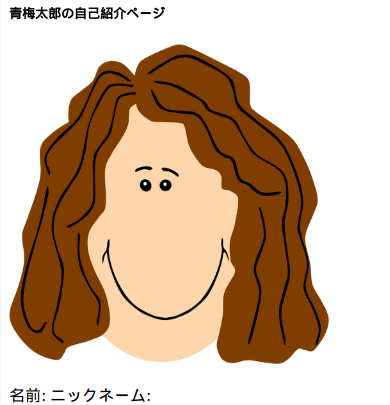
\includegraphics[width=5.373cm,height=5.579cm]{textbook-img228.png}
      &
      \centering
      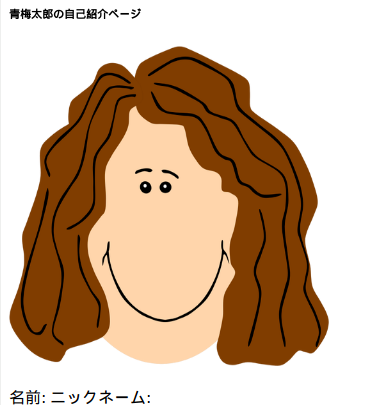
\includegraphics[width=5.373cm,height=5.579cm]{textbook-img229.png}
      &
      ~
      \\\hhline{--~}
      \centering h5 &
      \centering h6 &
      ~
      \\\hhline{--~}
    \end{supertabular}
  \end{center}

  h2〜h6にかけてじょじょに「青梅太郎の\ruby{自己}{じこ}紹介のページ」の文字が小さくなっている。
\end{minipage}
\clearpage\subsubsection{\bfseries
\ref*{Q:hasAnswer04-3}答え}

\centering
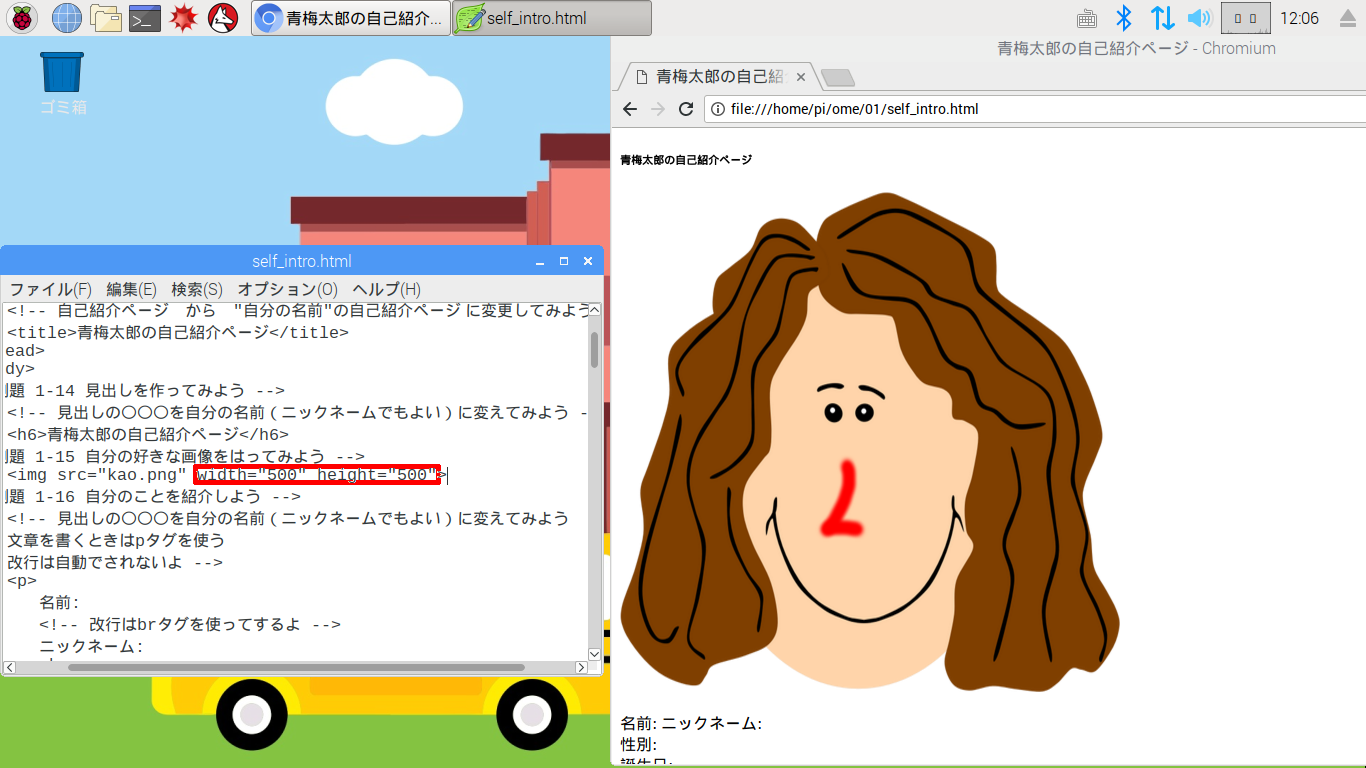
\includegraphics[width=11.591cm,height=6.516cm]{textbook-img230.png}
\flushleft
画像のサイズが変わっている。



\subsubsection{\bfseries
\ref*{Q:hasAnswer04-4}と\ref*{Q:hasAnswer04-5}の答え}

参考にして自分のページを作ろう。

\fbox{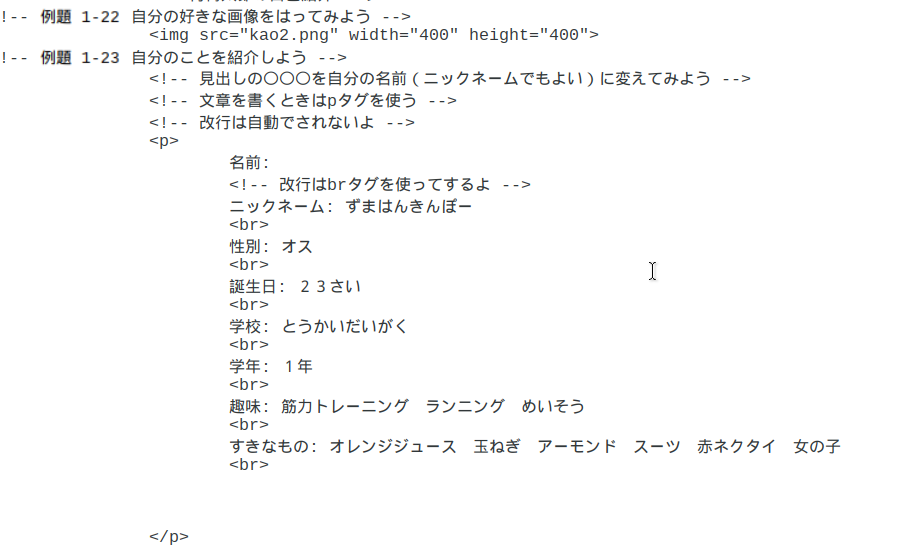
\includegraphics[width=11.118cm,height=6.706cm]{textbook-img231.png}}


\centering
\fbox{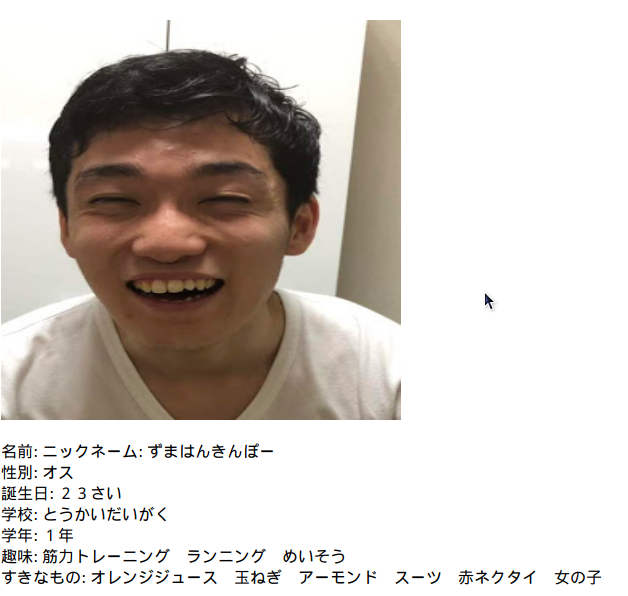
\includegraphics[width=7.354cm,height=6.98cm]{textbook-img232.png}}


\clearpage\subsubsection{\bfseries
\ref*{Q:hasAnswer04-6}答え}



\centering
\fbox{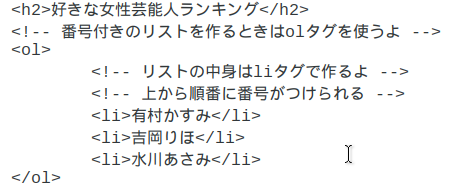
\includegraphics[width=8.245cm,height=3.225cm]{textbook-img233.png}}
\fbox{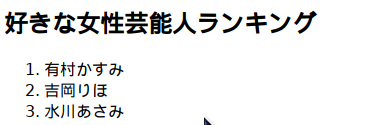
\includegraphics[width=7.422cm,height=2.535cm]{textbook-img234.png}}
\flushleft


参考にして自分のページを作ろう。

\subsubsection{\bfseries
\ref*{Q:hasAnswer04-7}答え}

ランキングではなく、\ruby{箇条}{かじょう}書きになる。

\centering
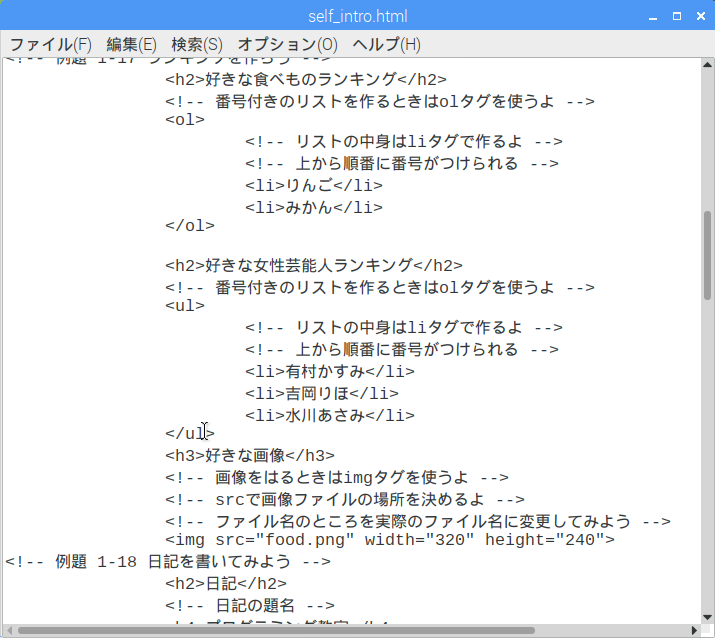
\includegraphics[width=7.622cm,height=6.8cm]{textbook-img236.png}
\fbox{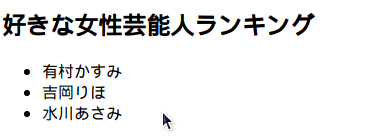
\includegraphics[width=7.904cm,height=2.805cm]{textbook-img235.png}}
\flushleft

\bigskip

\subsubsection{\bfseries
\ref*{Q:hasAnswer04-8}答え}



\centering
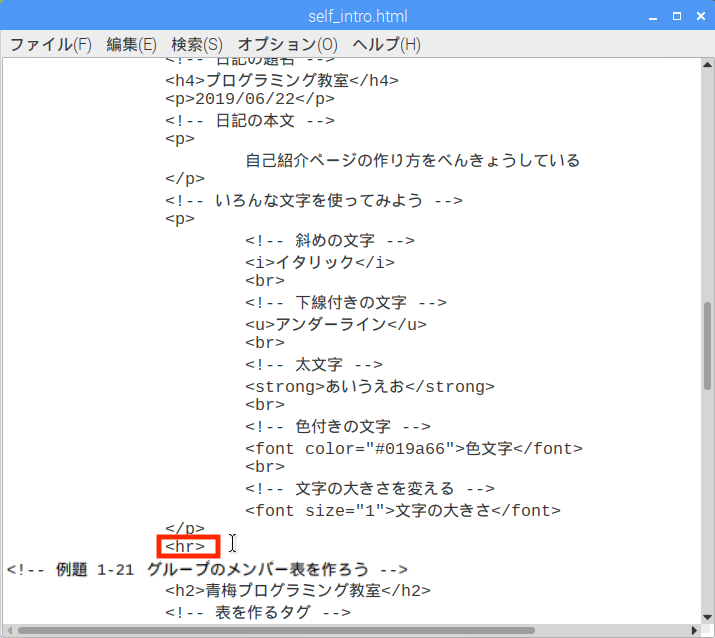
\includegraphics[width=8.186cm,height=7.304cm]{textbook-img237.png}
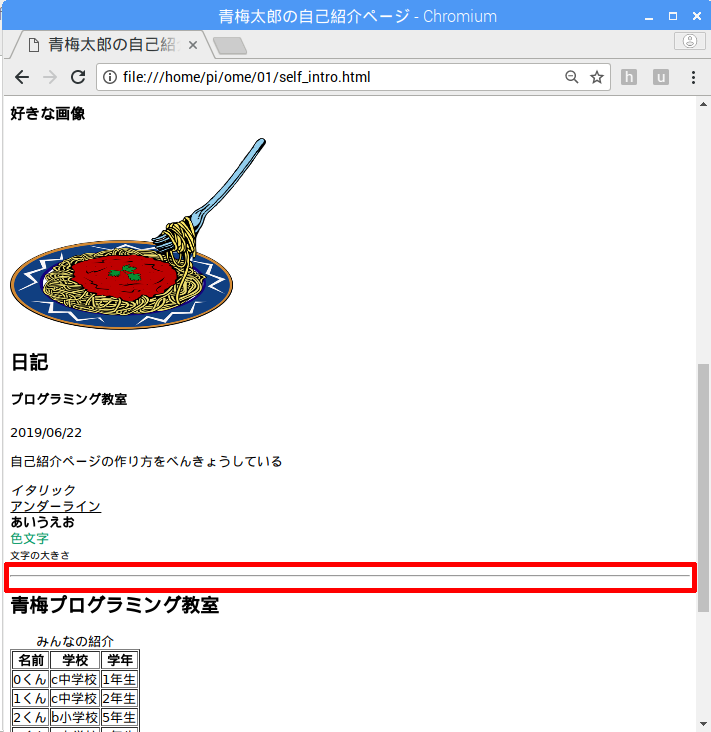
\includegraphics[width=7.163cm,height=7.373cm]{textbook-img238.png}
\flushleft

\bigskip


\bigskip

\clearpage\subsubsection{\bfseries
\ref*{Q:hasAnswer04-9}答え}



\centering
\fbox{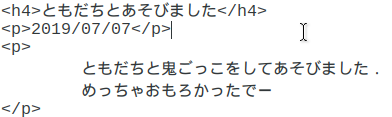
\includegraphics[width=9.938cm,height=2.967cm]{textbook-img239.png}}
\flushleft

\bigskip

\centering
\fbox{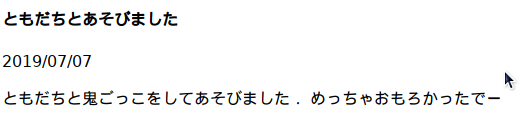
\includegraphics[width=14.048cm,height=3.149cm]{textbook-img240.png}}
\flushleft

\bigskip

参考にして自分のページを作ろう。


\bigskip

\subsubsection{\bfseries
\ref*{Q:hasAnswer04-10}答え}

%\newline

\centering
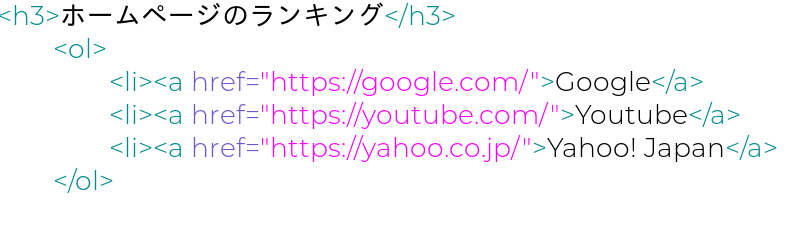
\includegraphics[width=12.448cm,height=3.129cm]{textbook-img241.png}
\flushleft

\bigskip

\centering
\fbox{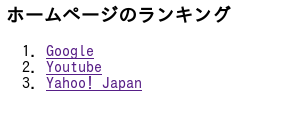
\includegraphics[width=8.331cm,height=3.044cm]{textbook-img242.png}}
\flushleft

\bigskip
参考にして自分のページを作ろう。

\clearpage\subsubsection{\bfseries
\ref*{Q:hasAnswer04-11}考え方}

%\liststyleLxxxii
\begin{enumerate}
  \item
        それぞれ画像をとります。\pageref*{E:webcam}ページの\ref*{E:webcam}を参考にしましょう。
  \item リストの\ruby{項目}{こうもく}をliタグで追加します。
  \item
        liタグのしたにimgタグを追加して画像を\ruby{表示}{ひょうじ}します。\pageref*{E:embImginHTML}ページの\ref*{E:embImginHTML}を参考にしましょう。
\end{enumerate}
\centering
\fbox{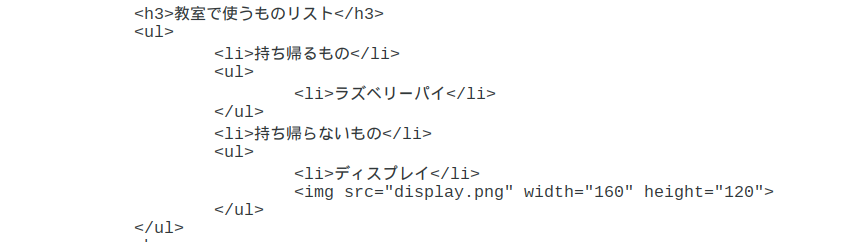
\includegraphics[width=13.407cm,height=4.822cm]{textbook-img243.png}}
\flushleft

\bigskip

\centering
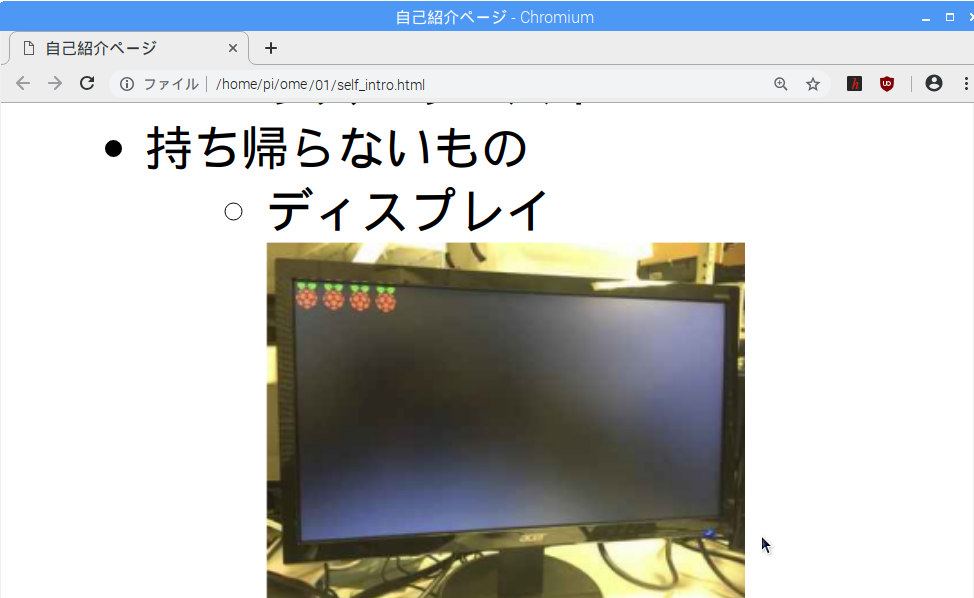
\includegraphics[width=17.006cm,height=10.44cm]{textbook-img244.png}
\flushleft

\bigskip

\clearpage
\end{document}